\section*{Funktionen}

\begin{multicols}{3}
    \subsection*{Lineare Funktion}
    \begin{center}
        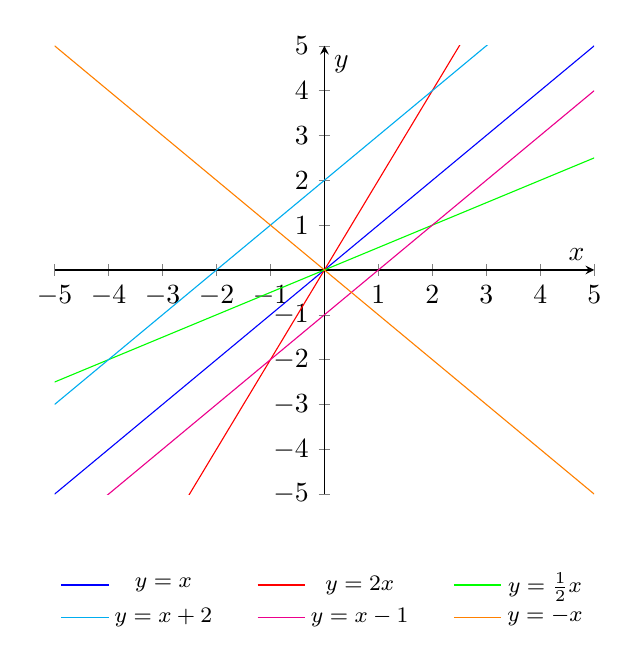
\begin{tikzpicture}
        \begin{axis}[
            axis lines=middle,
            xlabel=$x$,
            ylabel=$y$,
            xmin=-5,
            xmax=5,
            ymin=-5,
            ymax=5,
            xtick={-5,-4,-3,-2,-1,0,1,2,3,4,5},
            ytick={-5,-4,-3,-2,-1,0,1,2,3,4,5},
            legend pos=outer north east,
            legend style={
                draw=none,
                at={(0.5,-0.15)},
                anchor=north,
                legend columns=3,
                font=\footnotesize,
                /tikz/every even column/.append style={column sep=0.5cm},
            },
        ]
        
        % Linear Function: y = x
        \addplot[blue, domain=-5:5, samples=100] {x};
        \addlegendentry{$y = x$}
        
        % Transformed Functions
        \addplot[red, domain=-5:5, samples=100] {2*x};
        \addlegendentry{$y = 2x$}
        
        \addplot[green, domain=-5:5, samples=100] {0.5*x};
        \addlegendentry{$y = \frac{1}{2}x$}
        
        \addplot[cyan, domain=-5:5, samples=100] {x + 2};
        \addlegendentry{$y = x + 2$}
        
        \addplot[magenta, domain=-5:5, samples=100] {x - 1};
        \addlegendentry{$y = x - 1$}

        \addplot[orange, domain=-5:5, samples=100] {-x};
        \addlegendentry{$y = -x$}
        
        \end{axis}
        \end{tikzpicture}
    \end{center}
    \subsubsection*{Nullstelle berechnen}
    Funktion gleich Null setzen und nach X auflösen.
     \subsubsection*{Schnittpunkt berechnen}
    Beide Funktionen gleichsetzen, nach X auflösen und in eine der beiden Funktionen einsetzen um Y zu berechnen.

    \subsubsection*{Umkehrfunktion bilden}
    Funktion nach x auflösen, x und y vertauschen.
   
% Quadratic Function: y = x^2
\subsection*{Quadratische Funktion}
\begin{center}
    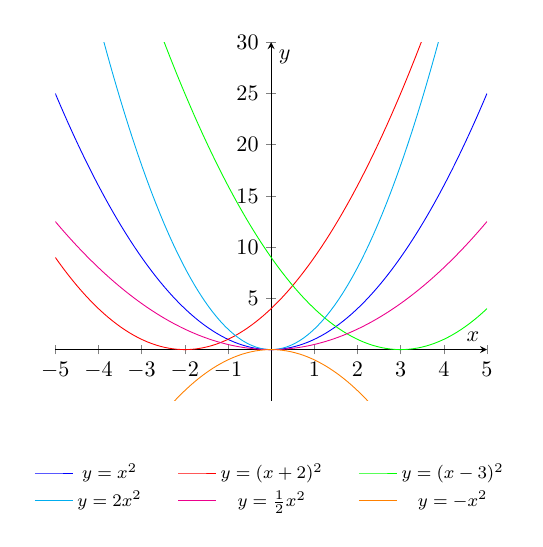
\begin{tikzpicture}[scale=0.8]
    \begin{axis}[
        axis lines=middle,
        xlabel=$x$,
        ylabel=$y$,
        xmin=-5,
        xmax=5,
        ymin=-5,
        ymax=30,
        xtick={-5,-4,-3,-2,-1,0,1,2,3,4,5},
        ytick={0,5,10,15,20,25,30},
        legend pos=outer north east,
            legend style={
                draw=none,
                at={(0.5,-0.15)},
                anchor=north,
                legend columns=3,
                font=\footnotesize,
                /tikz/every even column/.append style={column sep=0.5cm},
            },
    ]
    \addplot[blue, domain=-5:5, samples=100] {x^2};
    \addlegendentry{$y = x^2$}
    
    % Transformed Functions
    \addplot[red, domain=-5:5, samples=100] {(x+2)^2};
    \addlegendentry{$y = (x + 2)^2$}
    
    \addplot[green, domain=-5:5, samples=100] {(x-3)^2};
    \addlegendentry{$y = (x - 3)^2$}
    
    \addplot[cyan, domain=-5:5, samples=100] {2*x^2};
    \addlegendentry{$y = 2x^2$}
    
    \addplot[magenta, domain=-5:5, samples=100] {0.5*x^2};
    \addlegendentry{$y = \frac{1}{2}x^2$}

    \addplot[orange, domain=-5:5, samples=100] {-x^2};
    \addlegendentry{$y = -x^2$}
    
    \end{axis}
    \end{tikzpicture}
    \end{center}
    
    % Exponential Function: y = 2^x
    \subsection*{Exponential Funktion}
    \begin{center}
    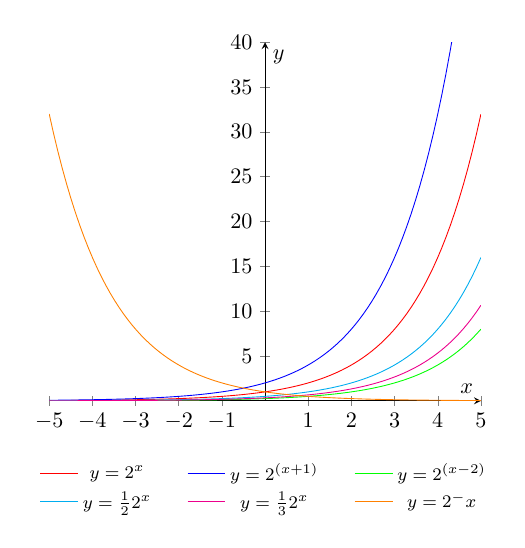
\begin{tikzpicture}[scale=0.8]
    \begin{axis}[
        axis lines=middle,
        xlabel=$x$,
        ylabel=$y$,
        xmin=-5,
        xmax=5,
        ymin=0,
        ymax=40,
        xtick={-5,-4,-3,-2,-1,0,1,2,3,4,5},
        ytick={0,5,10,15,20,25,30,35,40},
        legend pos=outer north east,
            legend style={
                draw=none,
                at={(0.5,-0.15)},
                anchor=north,
                legend columns=3,
                font=\footnotesize,
                /tikz/every even column/.append style={column sep=0.5cm},
            },
    ]
    \addplot[red, domain=-5:5, samples=100] {2^x};
    \addlegendentry{$y = 2^x$}
    
    % Transformed Functions
    \addplot[blue, domain=-5:5, samples=100] {2^(x+1)};
    \addlegendentry{$y = 2^{(x + 1)}$}
    
    \addplot[green, domain=-5:5, samples=100] {2^(x-2)};
    \addlegendentry{$y = 2^{(x - 2)}$}
    
    \addplot[cyan, domain=-5:5, samples=100] {0.5*2^x};
    \addlegendentry{$y = \frac{1}{2}2^x$}
    
    \addplot[magenta, domain=-5:5, samples=100] {2^x / 3};
    \addlegendentry{$y = \frac{1}{3}2^x$}

    \addplot[orange, domain=-5:5, samples=100] {2^-x};
    \addlegendentry{$y = 2^-x$}
    
    \end{axis}
    \end{tikzpicture}
    \end{center}
    
    \subsection*{Potenz Funktion}
    % Power Function: y = x^3
    \begin{center}
    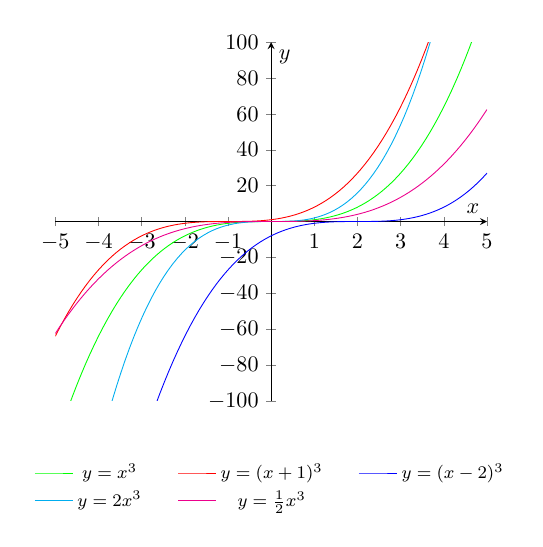
\begin{tikzpicture}[scale=0.8]
    \begin{axis}[
        axis lines=middle,
        xlabel=$x$,
        ylabel=$y$,
        xmin=-5,
        xmax=5,
        ymin=-100,
        ymax=100,
        xtick={-5,-4,-3,-2,-1,0,1,2,3,4,5},
        ytick={-100,-80,-60,-40,-20,0,20,40,60,80,100},
        legend pos=outer north east,
            legend style={
                draw=none,
                at={(0.5,-0.15)},
                anchor=north,
                legend columns=3,
                font=\footnotesize,
                /tikz/every even column/.append style={column sep=0.5cm},
            },
    ]
    \addplot[green, domain=-5:5, samples=100] {x^3};
    \addlegendentry{$y = x^3$}
    
    % Transformed Functions
    \addplot[red, domain=-5:5, samples=100] {(x+1)^3};
    \addlegendentry{$y = (x + 1)^3$}
    
    \addplot[blue, domain=-5:5, samples=100] {(x-2)^3};
    \addlegendentry{$y = (x - 2)^3$}
    
    \addplot[cyan, domain=-5:5, samples=100] {2*x^3};
    \addlegendentry{$y = 2x^3$}
    
    \addplot[magenta, domain=-5:5, samples=100] {0.5*x^3};
    \addlegendentry{$y = \frac{1}{2}x^3$}
    
    \end{axis}
    \end{tikzpicture}
    \end{center}
    
    \subsection*{Wurzel Funktion}
    % Square Root Function: y = sqrt(x)
    \begin{center}
    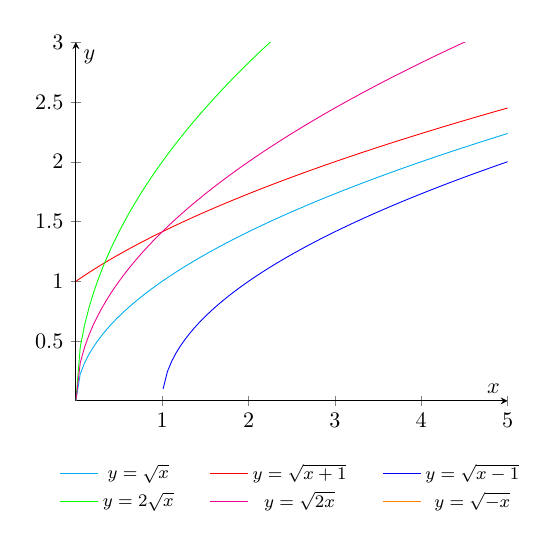
\begin{tikzpicture}[scale=0.8]
    \begin{axis}[
        axis lines=middle,
        xlabel=$x$,
        ylabel=$y$,
        xmin=0,
        xmax=5,
        ymin=0,
        ymax=3,
        xtick={0,1,2,3,4,5},
        ytick={0,0.5,1,1.5,2,2.5,3},
        legend pos=outer north east,
            legend style={
                draw=none,
                at={(0.5,-0.15)},
                anchor=north,
                legend columns=3,
                font=\footnotesize,
                /tikz/every even column/.append style={column sep=0.5cm},
            },
    ]
    \addplot[cyan, domain=0:5, samples=100] {sqrt(x)};
    \addlegendentry{$y = \sqrt{x}$}
    
    % Transformed Functions
    \addplot[red, domain=0:5, samples=100] {sqrt(x+1)};
    \addlegendentry{$y = \sqrt{x + 1}$}
    
    \addplot[blue, domain=0:5, samples=100] {sqrt(x-1)};
    \addlegendentry{$y = \sqrt{x - 1}$}
    
    \addplot[green, domain=0:5, samples=100] {2*sqrt(x)};
    \addlegendentry{$y = 2\sqrt{x}$}
    
    \addplot[magenta, domain=0:5, samples=100] {sqrt(2*x)};
    \addlegendentry{$y = \sqrt{2x}$}

    \addplot[orange, domain=0:5, samples=100] {sqrt(-x)};
    \addlegendentry{$y = \sqrt{-x}$}
    
    \end{axis}
    \end{tikzpicture}
    \end{center}
    
    \subsection*{Logarithmische Funktion}
    % Logarithmic Function: y = ln(x)
    \begin{center}
    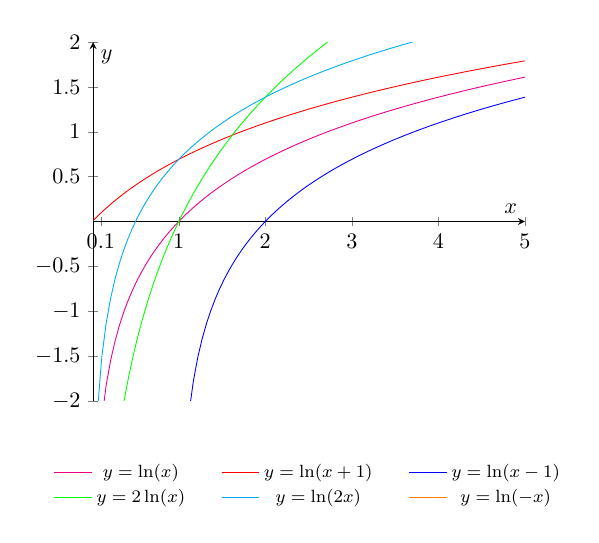
\begin{tikzpicture}[scale=0.8]
    \begin{axis}[
        axis lines=middle,
        xlabel=$x$,
        ylabel=$y$,
        xmin=0.01,
        xmax=5,
        ymin=-2,
        ymax=2,
        xtick={0.01,0.1,1,2,3,4,5},
        ytick={-2,-1.5,-1,-0.5,0,0.5,1,1.5,2},
        legend pos=outer north east,
            legend style={
                draw=none,
                at={(0.5,-0.15)},
                anchor=north,
                legend columns=3,
                font=\footnotesize,
                /tikz/every even column/.append style={column sep=0.5cm},
            },
    ]
    \addplot[magenta, domain=0.01:5, samples=100] {ln(x)};
    \addlegendentry{$y = \ln(x)$}
    
    % Transformed Functions
    \addplot[red, domain=0.01:5, samples=100] {ln(x+1)};
    \addlegendentry{$y = \ln(x + 1)$}
    
    \addplot[blue, domain=0.01:5, samples=100] {ln(x-1)};
    \addlegendentry{$y = \ln(x - 1)$}
    
    \addplot[green, domain=0.01:5, samples=100] {2*ln(x)};
    \addlegendentry{$y = 2\ln(x)$}
    
    \addplot[cyan, domain=0.01:5, samples=100] {ln(2*x)};
    \addlegendentry{$y = \ln(2x)$}

    \addplot[orange, samples=100] {ln(-x)};
    \addlegendentry{$y = \ln(-x)$}
    
    \end{axis}
    \end{tikzpicture}
    \end{center}
    \newpage
\end{multicols}